\begin{figure}[t]
    \centering
    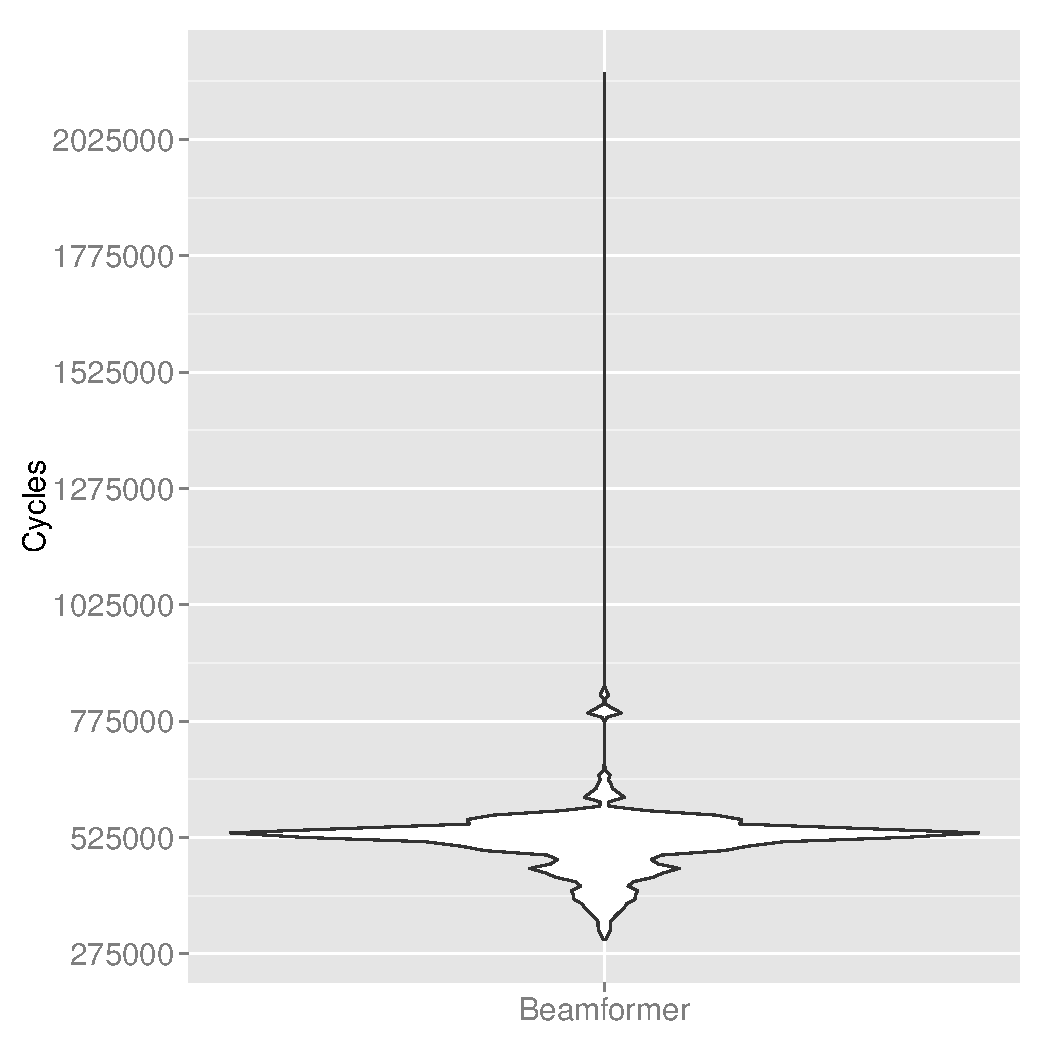
\includegraphics[width=1\textwidth]{streamit-paper/graphics/beamformer_motivation.pdf}
    \caption{Distribution of the runtime for Beamformer resulting from an exhaustively exploration of the hardware/software co-design space.
     The application has been partitioned into different number of threads and core compositions.}
     \label{fig:beamformermotiv}
\end{figure}

This section illustrates the difficulty of finding a good partition and resource allocation.
A simple experiment is conducted where one StreamIt benchmark is taken, \bench{Beamformer}, and partition its tasks into threads and allocate various number of cores to each thread.
A co-design of more than 32,000 combinations (exhaustive space) of thread mappings and core compositions is generated.
Each design point is executed on a dynamic multicore simulator (exact details about the experimental setup are presented later in section~\ref{sec:setup}).

Figure~\ref{fig:beamformermotiv} presents the distribution of the execution times from the co-design space as a violin plot.
For the unfamiliar reader, an intuitive way to think about this violin plot is to consider it as a smoothed histogram rotated by 90 degrees and mirrored.
The majority of the sampled points have a cycle count around 525,000 with the worst points taking more than 2 millions cycles.
The best performance is around 275,000 cycles which is about 2x faster than the majority of the data points.
This shows that finding the right combination of thread mapping and core composition is critical since a wrong choice often leads to suboptimal performance.

This example illustrates the necessity for designing the technique to predict both the optimal number of threads and core composition to use.
The next section will present a more in-depth analysis of the design space before presenting our machine-learning predictive model.

